\documentclass[8pt]{beamer}

\usetheme{metropolis}

\usepackage{pgfplots}
\usepackage{pgfplotstable}
\usepackage{varwidth}
\usepackage{xcolor}

\usetikzlibrary{arrows}
\usetikzlibrary{arrows.meta}
\usetikzlibrary{calc}

\date{19.01.23}
\title{Introduction to Machine Learning}
\author{Esten H. Leonardsenn}

\titlegraphic{
	\centering
	\vspace{7.5cm}
	
\includegraphics[height=1cm]{data/bio.png}
	\hfill
	
\includegraphics[height=1cm]{data/uio.png}
}

\def\nodesize{14pt}
\colorlet{nodefill}{green!20}

\begin{document}
	\begin{frame}
	 	\maketitle
	\end{frame}

	\begin{frame}{Terminologi} % Taxonomy, Artificial intelligence
		\centering
		\vfill
		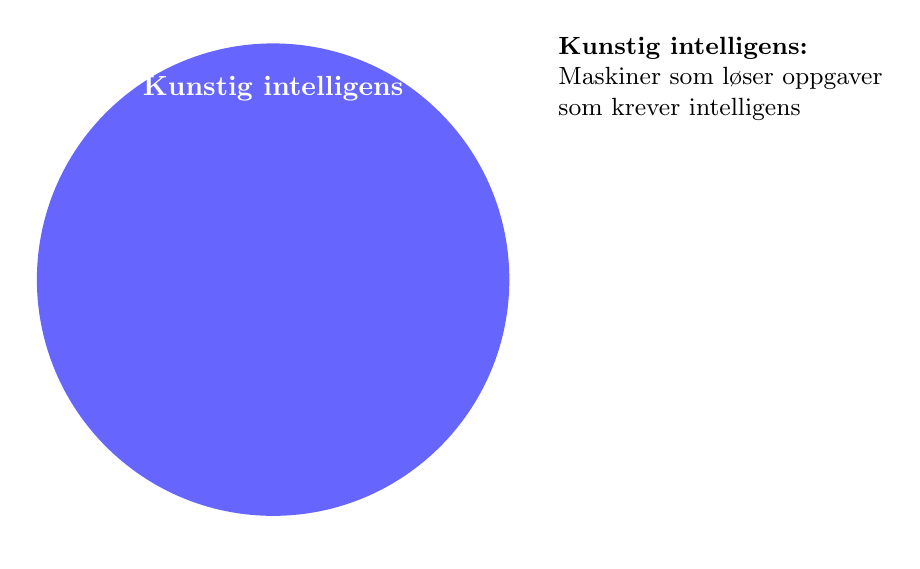
\begin{tikzpicture}
			\node[circle, fill=blue!60, minimum size=6cm] (ai) at (0, 0) {};
			\node[text=white, anchor=north] at ($ (ai.north) - (0, 0.3) $) {\textbf{Kunstig intelligens}};
			\node[anchor=north west, align=left, font=\small] (ai-text) at ($ (ai.north) + (3.5, 0.2) $) {\textbf{Kunstig intelligens:}\\Maskiner som løser oppgaver\\som krever intelligens};
			\node[] at (-3, 3) {};
			\node[] at (7.7, -3.2) {};
		\end{tikzpicture}
		\vfill
	\end{frame}

	\begin{frame}{Terminologi} % Taxonomy, Machine learning
		\centering
		\vfill
		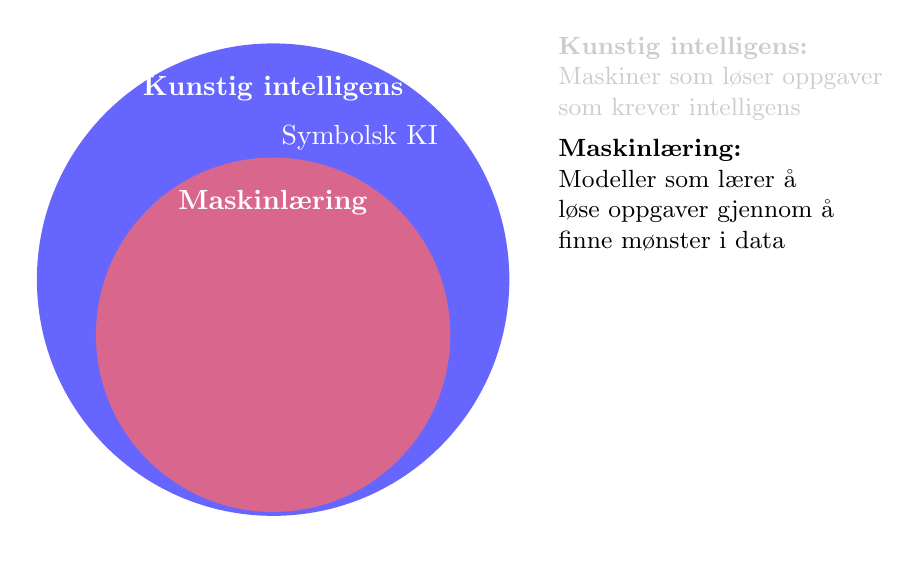
\begin{tikzpicture}
			\node[circle, fill=blue!60, minimum size=6cm] (ai) at (0, 0) {};
			\node[text=white, anchor=north] at ($ (ai.north) - (0, 0.3) $) {\textbf{Kunstig intelligens}};
			\node[text=white] at ($ (ai.north) - (-1.1, 1.2) $) {Symbolsk KI};
			\node[circle, fill=purple!60, minimum size=4.5cm, anchor=south] (ml) at ($ (ai.south) + (0, 0.05) $) {};
			\node[text=white, anchor=north] at ($ (ml.north) - (0, 0.3) $) {\textbf{Maskinlæring}};
			\node[anchor=north west, align=left, font=\small, text=gray!40] (ai-text) at ($ (ai.north) + (3.5, 0.2) $) {\textbf{Kunstig intelligens:}\\Maskiner som løser oppgaver\\som krever intelligens};
			\node[anchor=north west, align=left, font=\small] (ml-text) at ($ (ai-text.south west) - (0, 0) $) {\textbf{Maskinlæring:}\\Modeller som lærer å\\løse oppgaver gjennom å\\finne mønster i data};
			\node[] at (-3, 3) {};
			\node[] at (7.7, -3.2) {};
		\end{tikzpicture}
		\vfill
	\end{frame}

	\begin{frame}{Terminologi} % Taxonomy, Deep learning
		\centering
		\vfill
		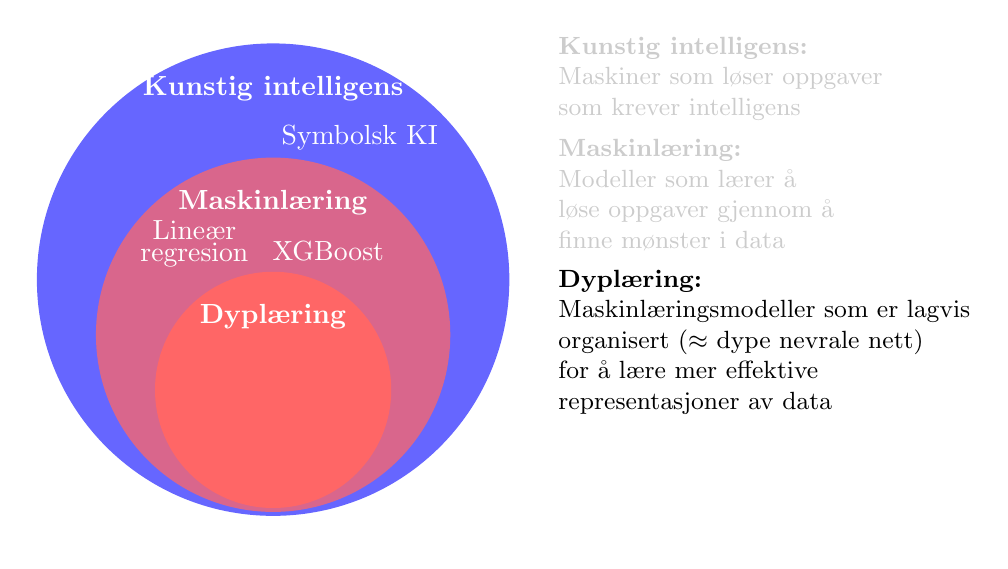
\begin{tikzpicture}
			\node[circle, fill=blue!60, minimum size=6cm] (ai) at (0, 0) {};
			\node[text=white, anchor=north] at ($ (ai.north) - (0, 0.3) $) {\textbf{Kunstig intelligens}};
			\node[text=white] at ($ (ai.north) - (-1.1, 1.2) $) {Symbolsk KI};
			\node[circle, fill=purple!60, minimum size=4.5cm, anchor=south] (ml) at ($ (ai.south) + (0, 0.05) $) {};
			\node[text=white, anchor=north] at ($ (ml.north) - (0, 0.3) $) {\textbf{Maskinlæring}};
			\node[text=white, align=center, font=\linespread{0.5}\selectfont] at ($ (ml.north) - (1, 1.1) $) {Lineær\\regresion};
			\node[text=white, align=center] at ($ (ml.north) - (-0.7, 1.2) $) {XGBoost};
			\node[circle, fill=red!60, minimum size=3cm, anchor=south] (dl) at ($ (ai.south) + (0, 0.1) $) {};
			\node[text=white, anchor=north] at ($ (dl.north) - (0, 0.3) $) {\textbf{Dyplæring}};
			\node[anchor=north west, align=left, font=\small, text=gray!40] (ai-text) at ($ (ai.north) + (3.5, 0.2) $) {\textbf{Kunstig intelligens:}\\Maskiner som løser oppgaver\\som krever intelligens};
			\node[anchor=north west, align=left, font=\small, text=gray!40] (ml-text) at ($ (ai-text.south west) - (0, 0) $) {\textbf{Maskinlæring:}\\Modeller som lærer å\\løse oppgaver gjennom å\\finne mønster i data};
			\node[anchor=north west, align=left, font=\small] (dl-text) at ($ (ml-text.south west) - (0, 0) $) {\textbf{Dyplæring:}\\Maskinlæringsmodeller som er lagvis\\ organisert ($\approx$ dype nevrale nett)\\for å lære mer effektive\\representasjoner av data};
			\node[] at (-3, 3) {};
			\node[] at (7.7, -3.2) {};
		\end{tikzpicture}
		\vfill
	\end{frame}

	\begin{frame}{Terminologi} % Taxonomy, CNNs and LLMs
		\centering
		\vfill
		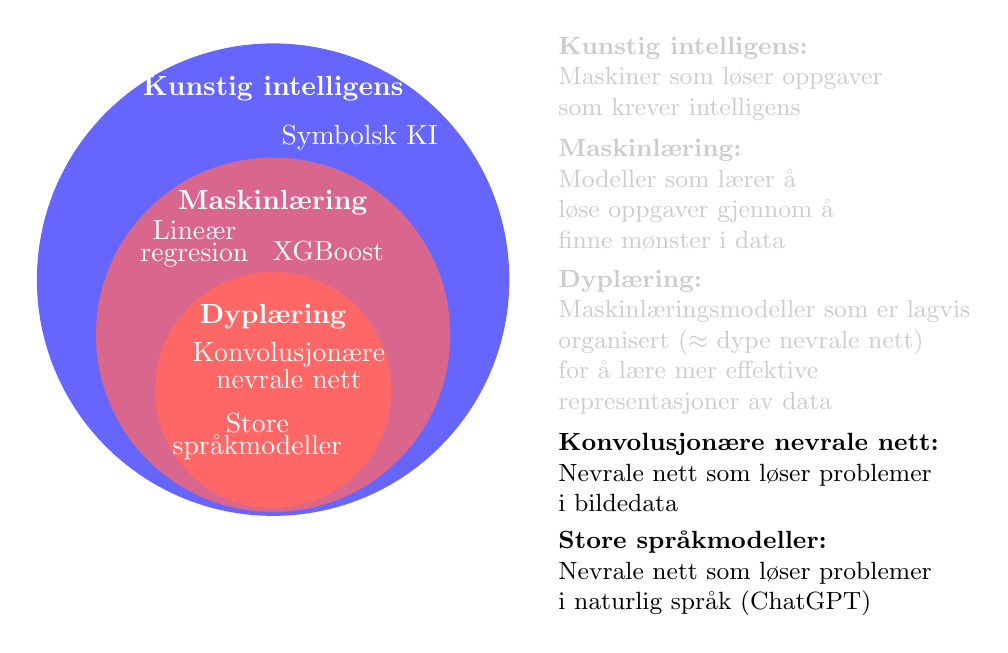
\begin{tikzpicture}
			\node[circle, fill=blue!60, minimum size=6cm] (ai) at (0, 0) {};
			\node[text=white, anchor=north] at ($ (ai.north) - (0, 0.3) $) {\textbf{Kunstig intelligens}};
			\node[text=white] at ($ (ai.north) - (-1.1, 1.2) $) {Symbolsk KI};
			\node[circle, fill=purple!60, minimum size=4.5cm, anchor=south] (ml) at ($ (ai.south) + (0, 0.05) $) {};
			\node[text=white, anchor=north] at ($ (ml.north) - (0, 0.3) $) {\textbf{Maskinlæring}};
			\node[text=white, align=center, font=\linespread{0.5}\selectfont] at ($ (ml.north) - (1, 1.1) $) {Lineær\\regresion};
			\node[text=white, align=center] at ($ (ml.north) - (-0.7, 1.2) $) {XGBoost};
			\node[circle, fill=red!60, minimum size=3cm, anchor=south] (dl) at ($ (ai.south) + (0, 0.1) $) {};
			\node[text=white, anchor=north] at ($ (dl.north) - (0, 0.3) $) {\textbf{Dyplæring}};
			\node[align=center, text=white, font=\linespread{0.5}\selectfont] at ($ (dl.north) - (-0.2, 1.2) $) {Konvolusjonære\\nevrale nett};
			\node[align=center, text=white, font=\linespread{0.5}\selectfont] at ($ (dl.north) - (0.2, 2.1) $) {Store\\språkmodeller};
			\node[anchor=north west, align=left, font=\small, text=gray!40] (ai-text) at ($ (ai.north) + (3.5, 0.2) $) {\textbf{Kunstig intelligens:}\\Maskiner som løser oppgaver\\som krever intelligens};
			\node[anchor=north west, align=left, font=\small, text=gray!40] (ml-text) at ($ (ai-text.south west) - (0, 0) $) {\textbf{Maskinlæring:}\\Modeller som lærer å\\løse oppgaver gjennom å\\finne mønster i data};
			\node[anchor=north west, align=left, font=\small, text=gray!40] (dl-text) at ($ (ml-text.south west) - (0, 0) $) {\textbf{Dyplæring:}\\Maskinlæringsmodeller som er lagvis\\ organisert ($\approx$ dype nevrale nett)\\for å lære mer effektive\\representasjoner av data};
			\node[anchor=north west, align=left, font=\small] (cnn-text) at ($ (dl-text.south west) - (0, 0) $) {\textbf{Konvolusjonære nevrale nett:}\\Nevrale nett som løser problemer\\i bildedata};
			\node[anchor=north west, align=left, font=\small] at ($ (cnn-text.south west) - (0, 0) $) {\textbf{Store språkmodeller:}\\Nevrale nett som løser problemer\\i naturlig språk (ChatGPT)};
			\node[] at (-3, 3) {};
			\node[] at (7.7, -3.2) {};
		\end{tikzpicture}
		\vfill
	\end{frame}

	\begin{frame}{Terminologi} % Sterk vs svak, dikotomi
		\centering
		\vfill
		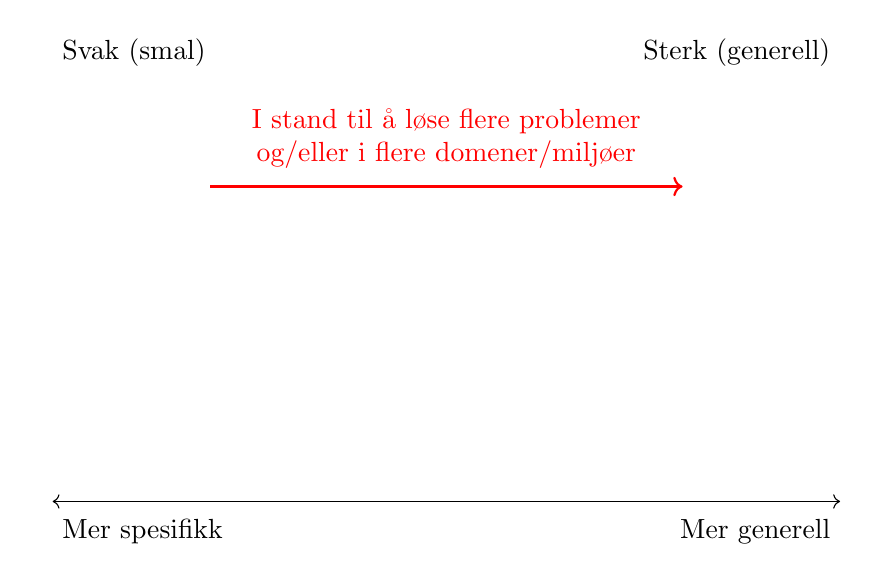
\begin{tikzpicture}
			\draw[<->] (0, 0) -- (10, 0);
			\node[anchor=north west] at (0, -0.1) {Mer spesifikk};
			\node[anchor=north east] at (10, -0.1) {Mer generell};
			\node[anchor=north west] at (0, 6) {Svak (smal)};
			\node[anchor=north east] at (10, 6) {Sterk (generell)};

			\draw[red, ->, thick] (2, 4) -- (8, 4);
			\node[anchor=south,align=center,text=red] at (5, 4.1) {I stand til å løse flere problemer\\og/eller i flere domener/miljøer};

			\node[] at (10.2, -0.4) {};
			\node[] at (-0.2, 5.9) {};
		\end{tikzpicture}
		\vfill
	\end{frame}

	\begin{frame}{Terminologi} % Sterk vs svak, dikotomi
		\centering
		\vfill
		\begin{tikzpicture}
			\draw[<->] (0, 0) -- (10, 0);
			\node[anchor=north west] at (0, -0.1) {Mer spesifikk};
			\node[anchor=north east] at (10, -0.1) {Mer generell};
			\node[anchor=north west] at (0, 6) {Svak (smal)};
			\node[anchor=north east] at (10, 6) {Sterk (generell)};

			\draw[red, ->, thick] (2, 4) -- (8, 4);
			\node[anchor=south,align=center,text=red] at (5, 4.1) {I stand til å løse flere problemer\\og/eller i flere domener/miljøer};
			\node[anchor=south east] at (9.5, 0.2) {
				
\includegraphics[width=1.3cm]{data/human.png}
			};
			\node[anchor=south west] at (0.5, 0.2) {
				
\includegraphics[width=1.3cm]{data/laptop.png}
			};
			\node[] at (10.2, -0.4) {};
			\node[] at (-0.2, 5.9) {};
		\end{tikzpicture}
		\vfill
	\end{frame}

	\begin{frame}{Terminologi} % Sterk vs svak, svake
		\centering
		\vfill
		\begin{tikzpicture}
			\draw[<->] (0, 0) -- (10, 0);
			\node[anchor=north west] at (0, -0.1) {Mer spesifikk};
			\node[anchor=north east] at (10, -0.1) {Mer generell};
			\node[anchor=north west] at (0, 6) {Svak (smal)};
			\node[anchor=north east] at (10, 6) {Sterk (generell)};

			\draw[red, ->, thick] (2, 4) -- (8, 4);
			\node[anchor=south,align=center,text=red] at (5, 4.1) {I stand til å løse flere problemer\\og/eller i flere domener/miljøer};
			\node[anchor=south east] at (9.5, 0.2) {
				
\includegraphics[width=1.3cm]{data/human.png}
			};
			\node[anchor=south west] at (0.5, 0.2) {
				
\includegraphics[width=1.3cm]{data/laptop.png}
			};
			\node[align=center,font=\small, fill=blue!60, text=white, minimum width=1.6cm, rounded corners=.1cm] at (3, 2.1) {
				Bilde-\\
				diagnostikk
			};
			\node[align=center,font=\small, fill=blue!60, text=white, minimum width=1.6cm, rounded corners=.1cm] at (3, 1.3) {
				Forsikrings-\\
				prising
			};
			\node[align=center,font=\small, fill=blue!60, text=white, minimum width=1.6cm, rounded corners=.1cm] at (3, 0.5) {
				Dokument-\\
				lesing
			};
			\node[] at (10.2, -0.4) {};
			\node[] at (-0.2, 5.9) {};
		\end{tikzpicture}
		\vfill
	\end{frame}

	\begin{frame}{Terminologi} % Sterk vs svak, svake
		\centering
		\vfill
		\begin{tikzpicture}
			\draw[<->] (0, 0) -- (10, 0);
			\node[anchor=north west] at (0, -0.1) {Mer spesifikk};
			\node[anchor=north east] at (10, -0.1) {Mer generell};
			\node[anchor=north west] at (0, 6) {Svak (smal)};
			\node[anchor=north east] at (10, 6) {Sterk (generell)};

			\draw[red, ->, thick] (2, 4) -- (8, 4);
			\node[anchor=south,align=center,text=red] at (5, 4.1) {I stand til å løse flere problemer\\og/eller i flere domener/miljøer};
			\node[anchor=south east] at (9.5, 0.2) {
				
\includegraphics[width=1.3cm]{data/human.png}
			};
			\node[anchor=south west] at (0.5, 0.2) {
				
\includegraphics[width=1.3cm]{data/laptop.png}
			};
			\node[align=center,font=\small, fill=blue!60, text=white, minimum width=1.6cm, rounded corners=.1cm] at (3, 2.1) {
				Bilde-\\
				diagnostikk
			};
			\node[align=center,font=\small, fill=blue!60, text=white, minimum width=1.6cm, rounded corners=.1cm] at (3, 1.3) {
				Forsikrings-\\
				prising
			};
			\node[align=center,font=\small, fill=blue!60, text=white, minimum width=1.6cm, rounded corners=.1cm] at (3, 0.5) {
				Dokument-\\
				lesing
			};
			\node[align=center,font=\small, fill=blue!60, text=white, minimum width=1.6cm, rounded corners=.1cm] at (4.8, 0.5) {
				Tesla
			};
			\node[align=center,font=\small, fill=blue!60, text=white, minimum width=1.6cm, rounded corners=.1cm] at (5.4, 1.1) {
				ChatGPT
			};
			\node[] at (10.2, -0.4) {};
			\node[] at (-0.2, 5.9) {};
		\end{tikzpicture}
		\vfill
	\end{frame}

	\begin{frame}{Terminologi}
		\centering
		\vfill
		\begin{tikzpicture}
			\node[align=center, anchor=north] (supervised) at (0, 0) {Veiledet læring\\(Supervised learning)};
			\node[align=center, anchor=north] (unsupervised) at (7, 0) {Ikke-veiledet læring\\(Unsupervised learning)};
			\draw[dashed] (3.5, 0) -- (3.5, -7);
		\end{tikzpicture}
		\vfill
	\end{frame}
\end{document}
